\lesson{6}{Mar 04 2022 Fri (21:13:37)}{Solve quadratic inequality}{Unit 4}

Let's say we have $x^{2} -x \ge 12$. When dealing with an equation where $x =
a$, $x$ has a set value. But if you're dealing with an inequality, $x$ has a
range of values.

\begin{equation}
  \label{e qt:solving_quadratic_inequality}
  \begin{alignedat}{2}
    x^{2} - x - 12 &\ge 12 \qquad\qquad &&\textrm{Set everything to $0$} \\
    (x - 4)(x + 3) &\ge 12 \qquad\qquad&& \textrm{Factor the quadratic} \\
    x &= 4, -3 \qquad\qquad&& \textrm{Find the roots} \\
  \end{alignedat}
.\end{equation}

Since the solution includes $4 \qquad\qquad -3$, we're going to put filled
circles at those points on a number line.

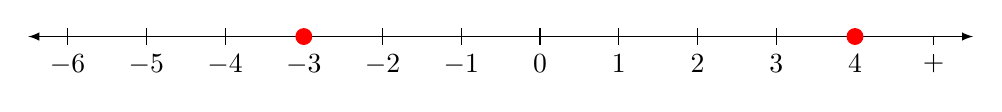
\begin{tikzpicture}
  \draw[latex-latex] (-6.5,0) -- (5.5,0);
  \foreach \x in {-6,-5,-4,-3,-2,-1,0,1,2,3,4}
  \draw[shift={(\x,0)},color=black] (0pt,3pt) -- (0pt,-3pt);
  \foreach \x in {-6,-5,-4,-3,-2,-1,0,1,2,3,4}
  \draw[shift={(\x,0)},color=black] (0pt,0pt) -- (0pt,-3pt) node[below] 
  {$\x$};
  \foreach \x in {5}
  \draw[shift={(\x,0)},color=black] (0pt,0pt) -- (0pt,-3pt) node[below] 
  {+};

  \draw [red,fill=red,radius=0.1] (4,0) circle;
  \draw [red,fill=red,radius=0.1] (-3,0) circle;
\end{tikzpicture}

Since it's $\ge 0$, we need to check the $3$ regions that's in between the
points to see if it's positive. So, we got to plugin numbers and test the signs.

Let's plug-in $5$ into the expression: $(x - 4)(x + 3) \ge 0$:

\begin{equation}
  \label{eqt:check_signs}
  \begin{split}
    (x - 4)(x + 3) &\ge 0 \\
    1(8) &= 8 \qquad\qquad \textrm{Which is $> 0$} \\
  \end{split}
.\end{equation}

Now, we need to check a number that's between $-3$ and $4$. Let's go with $0$.

\begin{equation}
  \label{eqt:check_signs}
  \begin{split}
    (x - 4)(x + 3) &\ge 0 \\
    -4(3) &= -12 \qquad\qquad \textrm{Which is $< 0$} \\
  \end{split}
.\end{equation}

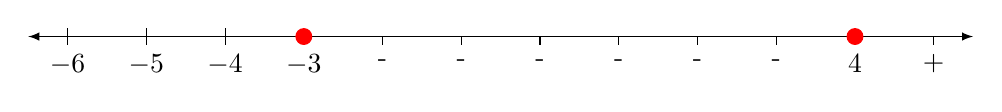
\begin{tikzpicture}
  \draw[latex-latex] (-6.5,0) -- (5.5,0);
  \foreach \x in {-6,-5,-4,-3,4}
  \draw[shift={(\x,0)},color=black] (0pt,3pt) -- (0pt,-3pt);
  \foreach \x in {-6,-5,-4,-3,4}
  \draw[shift={(\x,0)},color=black] (0pt,0pt) -- (0pt,-3pt) node[below] 
  {$\x$};
  \foreach \x in {5}
  \draw[shift={(\x,0)},color=black] (0pt,0pt) -- (0pt,-3pt) node[below] 
  {+};
  \foreach \x in {-2,-1,0,1,2,3}
  \draw[shift={(\x,0)},color=black] (0pt,0pt) -- (0pt,-3pt) node[below] 
  {-};

  \draw [red,fill=red,radius=0.1] (4,0) circle;
  \draw [red,fill=red,radius=0.1] (-3,0) circle;
\end{tikzpicture}

Now, we need to check a number that's greater than $-3$. Let's go with $-4$.

\begin{equation}
  \label{eqt:check_signs}
  \begin{split}
    (x - 4)(x + 3) &\ge 0 \\
    -8(-1) &= 8 \qquad\qquad \textrm{Which is $> 0$} \\
  \end{split}
.\end{equation}

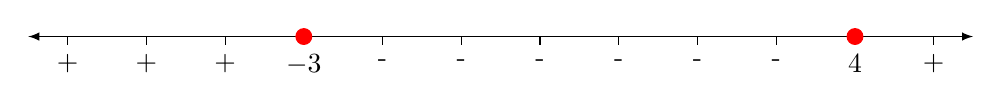
\begin{tikzpicture}
  \draw[latex-latex] (-6.5,0) -- (5.5,0);
  \foreach \x in {-3,4}
  \draw[shift={(\x,0)},color=black] (0pt,3pt) -- (0pt,-3pt);
  \foreach \x in {-3,4}
  \draw[shift={(\x,0)},color=black] (0pt,0pt) -- (0pt,-3pt) node[below] 
  {$\x$};
  \foreach \x in {5}
  \draw[shift={(\x,0)},color=black] (0pt,0pt) -- (0pt,-3pt) node[below] 
  {+};
  \foreach \x in {-2,-1,0,1,2,3}
  \draw[shift={(\x,0)},color=black] (0pt,0pt) -- (0pt,-3pt) node[below] 
  {-};
  \foreach \x in {-6,-5,-4}
  \draw[shift={(\x,0)},color=black] (0pt,0pt) -- (0pt,-3pt) node[below] 
  {+};

  \draw [red,fill=red,radius=0.1] (4,0) circle;
  \draw [red,fill=red,radius=0.1] (-3,0) circle;
\end{tikzpicture}

Here's a quicker method. Take a look at the multiplicity of the factored
quadratic: $(x - 4)^{1}(x + 3)^{1}$. When the multiplicity is odd, the sign will
change at that point. So, if you know the first sign, you can easily determine
the rest. So, for the zero $4$, the multiplicity is odd, so, it's going to
switch from $+$ to $-$. And for the zero $3$, the multiplicity is odd, so it's
going to switch from  $-$ to $+$.

Here's the final graphed answer:

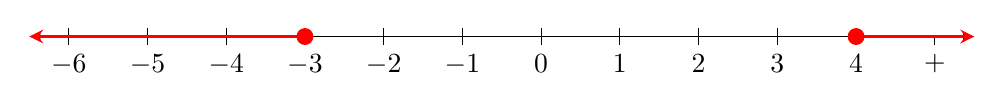
\begin{tikzpicture}
  \draw[latex-latex] (-6.5,0) -- (5.5,0);
  \foreach \x in {-6,-5,-4,-3,-2,-1,0,1,2,3,4}
  \draw[shift={(\x,0)},color=black] (0pt,3pt) -- (0pt,-3pt);
  \foreach \x in {-6,-5,-4,-3,-2,-1,0,1,2,3,4}
  \draw[shift={(\x,0)},color=black] (0pt,0pt) -- (0pt,-3pt) node[below] 
  {$\x$};
  \foreach \x in {5}
  \draw[shift={(\x,0)},color=black] (0pt,0pt) -- (0pt,-3pt) node[below] 
  {+};

  \draw [red,fill=red,radius=0.1] (4,0) circle;
  \draw [red,fill=red,radius=0.1] (-3,0) circle;

  \draw [-stealth,red,very thick] (4,0) -- (5.5,0);
  \draw [-stealth,red,very thick] (-3,0) -- (-6.5,0);

\end{tikzpicture}

And here's the final answer in interval notation:

\begin{equation}
  \label{eqt:final_answer_in_interval_notation}
  \begin{split}
    (-\infty, -3]\cup[4,\infty) \qquad\qquad \textrm{or} \qquad\qquad
    x \le -3 \qquad \textrm{or} \qquad x \ge 4 \\
  \end{split}
.\end{equation}

\newpage
